\documentclass[12pt]{article}%
%Options -- Point size:  10pt (default), 11pt, 12pt
%        -- Paper size:  letterpaper (default), a4paper, a5paper, b5paper
%                        legalpaper, executivepaper
%        -- Orientation  (portrait is the default)
%                        landscape
%        -- Print size:  oneside (default), twoside
%        -- Quality      final(default), draft
%        -- Title page   notitlepage, titlepage(default)
%        -- Columns      onecolumn(default), twocolumn
%        -- Equation numbering (equation numbers on the right is the default)
%                        leqno
%        -- Displayed equations (centered is the default)
%                        fleqn (equations start at the same distance from the right side)
%        -- Open bibliography style (closed is the default)
%                        openbib

% general layout
\usepackage[dvips,letterpaper,margin=0.75in,bottom=0.75in]{geometry}
\usepackage{rotating}
%\usepackage{multicol}
\setlength{\parindent}{0pt}
\usepackage{setspace} % line spacing
\usepackage{changepage}

%\pagestyle{empty} % Removes page numbers
%\pagestyle{plain} 
\usepackage{fancyhdr}
\usepackage{lastpage}
\usepackage{extramarks}

% Setup the header and footer
\newcommand{\hmwkAuthorName}{Colin Leach}
\fancyhf{}
\pagestyle{fancy}                                                       %
\lhead{\hmwkAuthorName}                                                 %
\chead{\hmwkClass\ : \hmwkTitle}  %
\rhead{Page\ \thepage\ of\ \pageref{LastPage}}                          %
\renewcommand\headrulewidth{0.4pt}                                      %
\renewcommand\footrulewidth{0pt}                                      %

% Make title
\title{\vspace{-1cm}\textmd{\textbf{\hmwkClass:\ \hmwkTitle}}\\\normalsize\vspace{0.1in}\small{Due\ on\ \hmwkDueDate}\\\vspace{0.1in}}
\date{}
\author{\textbf{\hmwkAuthorName}}\vspace{-0.2in}

% base encodings
\usepackage[utf8]{inputenc}
\usepackage[T1]{fontenc}

% math support packages
\usepackage{amsmath}
\usepackage{amsfonts}
\usepackage{amssymb}
\usepackage{mathabx}
%\usepackage[retainorgcmds]{IEEEtran} % problems installing with MikTeX
\DeclareMathOperator{\tr}{tr} % trace of a matrix
\usepackage{mathptmx}
%\usepackage{newtxmath}
\usepackage{bm} % bold math
%\usepackage{commath}
\usepackage{mathtools}
\usepackage{upgreek}
\DeclareMathAlphabet{\mathcal}{OMS}{cmsy}{m}{n}


% graphics-related packages and settings
\usepackage{graphicx}
\graphicspath{ {images/} }
\usepackage{wrapfig} % allow text to wrap around (narrow) figures
%\usepackage{float} % do not use with floatrow
\usepackage{floatrow} % allow floats and captions side by side
\usepackage[font=small,labelfont=bf,labelsep=space,justification=raggedright]{caption}
\usepackage{chngcntr} % defines \counterwithin and \counterwithout
\counterwithin{figure}{section}

% table formatting
\usepackage{makecell}
\usepackage[table]{xcolor}
\usepackage{array} % wrap within tables
\newcolumntype{L}{>{\centering\arraybackslash}m{12cm}}

% miscellaneous
\usepackage{subfiles} % include source from separate files
\usepackage{hyperref} % hypertext support
\usepackage{color}
\usepackage[bottom]{footmisc}
\newcommand{\tsub}[1]{\textsubscript{#1}}
\newcommand{\tsup}[1]{\textsuperscript{#1}}
\newcommand{\so}{\qquad \implies \qquad}
\newcommand{\todo}{\color{red}{TODO}\color{black}\hspace{2mm}}

% for software source code
% Python, Matlab, etc are built in as atandard but Julia needs to be added here
\usepackage{listings}
%%
%% Julia definition (c) 2014 Jubobs
%%
\lstdefinelanguage{Julia} 
{morekeywords={abstract,break,case,catch,const,continue,do,else,elseif,%
		end,export,false,for,function,immutable,import,importall,if,in,%
		macro,module,otherwise,quote,return,switch,true,try,type,typealias,%
		using,while},%
	sensitive=true,%
	alsoother={$},%
	morecomment=[l]\#,%
	morecomment=[n]{\#=}{=\#},%
	morestring=[s]{"}{"},%
	morestring=[m]{'}{'},%
}[keywords,comments,strings]%






%\setlength{\headsep}{-10pt}
\setlength{\parskip}{0.05em}
%\setlength{\textheight}{11 in}
\setlength{\skip\footins}{20pt}

% Homework Specific Information
\newcommand{\hmwkClass}{ASTR 400B}
\newcommand{\hmwkTitle}{Homework 6}
\newcommand{\hmwkDueDate}{March 6, 2020}

\hyphenpenalty=1000

\begin{document}
	
\maketitle

Calculations are in ./OrbitCOM.ipynb, this is just a summary.

\section*{1) CoM Relative Motion Plots}

{\centering 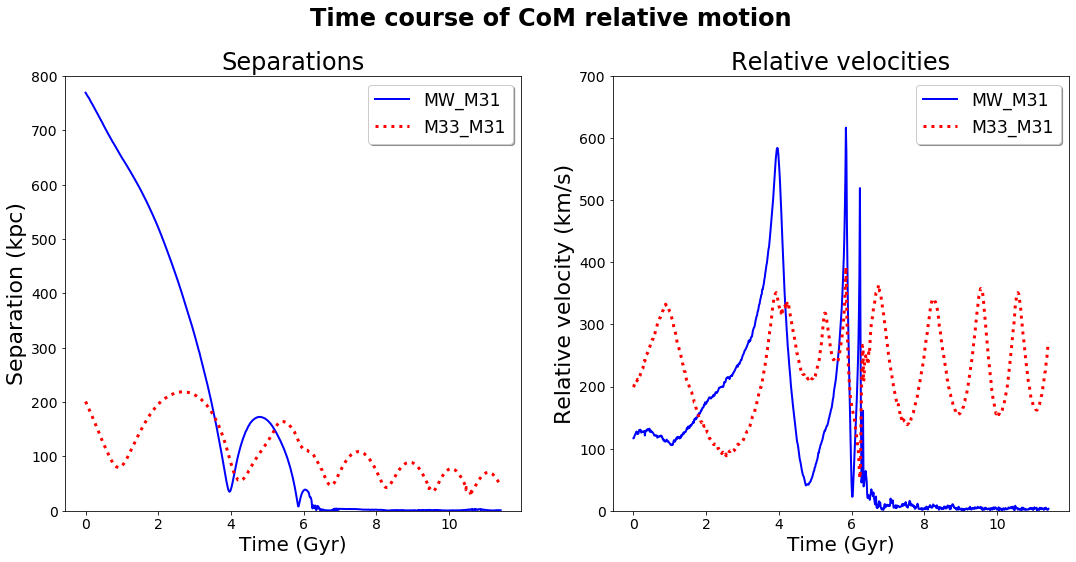
\includegraphics[scale=0.43]{all_pos_v} \par}

\section*{2) Close Encounters and Merger, MW-M31}

This is a bit hard to see in the graphs above (left subplot, blue line). For better mouse interactivity it was redrawn in Plotly:

{\centering 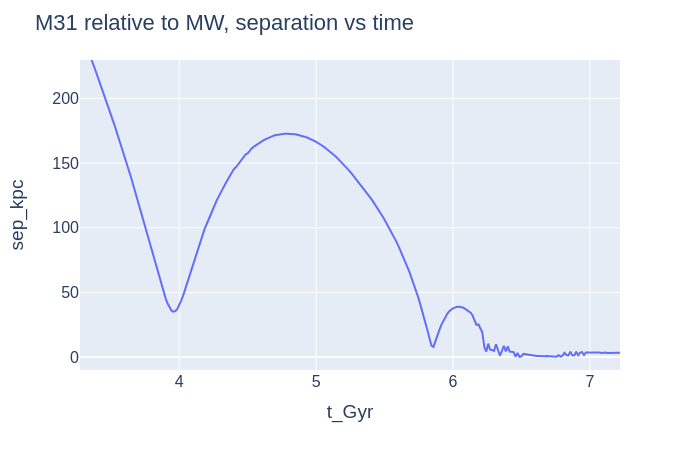
\includegraphics[scale=0.42]{M31_MW_zoom} \par}

How many close encounters do we expect? It depends a bit on definitions:
\begin{itemize}
	\setlength\itemsep{0pt}
	\item at 4.8 Gyr there is a relatively benign encounter
	\item just after 6.0 Gyr there is a closer and more disruptive encounter, after which the galaxies barely separate
	\item merger happens at about 6.2 Gyr (a \textit{very} close encounter?)
\end{itemize}

What do these look like in 3D? This definitely needs to be viewed in the browser, from many directions, but these are two attempts to make a static visualization:

{\centering 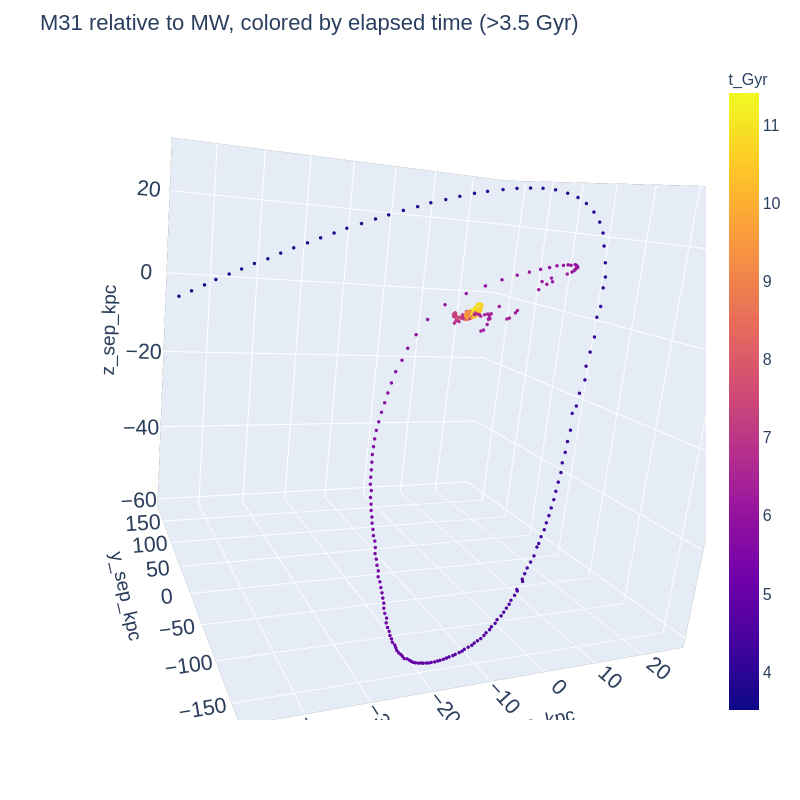
\includegraphics[scale=0.3]{M31_MW_3d_time}  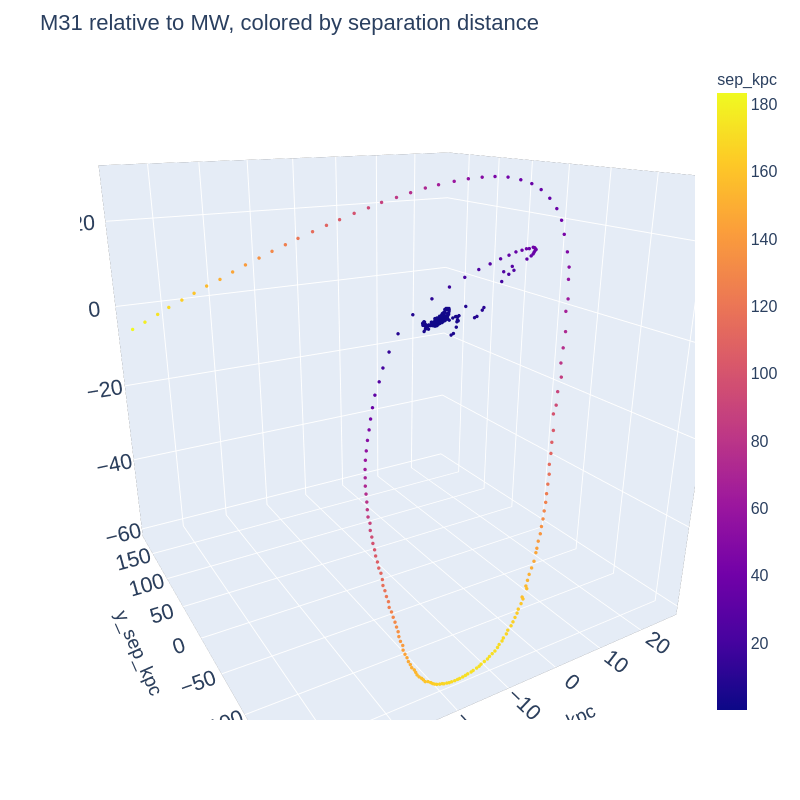
\includegraphics[scale=0.3]{M31_MW_3d_sep} \par}

In both cases, points are plotted at 1 Myr intervals, starting from 3.5 Gyr. In the left plot they are colored by elapsed time, in the right plot by separation. It's complicated...

\section*{3) Separation vs Velocity}

The overall trend is for higher relative velocities at smaller separations, somewhat like a Keplerian orbit of high ellipticity. However, it's not nearly as simple in this case. Points are plotted in time order, starting on the right at about 2.8 Gyr:

{\centering 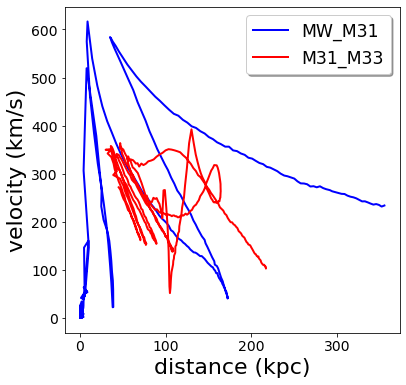
\includegraphics[scale=0.5]{pos_vel} \par}



\section*{4) M33-M31 Merger}

The galaxies reach apocenter at [2.657, 5.414, 7.50, 8.914, 10.057, 11.057] Gyr. Separation falls monotonically at successive orbits (red curves) and unsurprisingly so does the orbital period (blue curve).\vspace{5mm}

{\centering 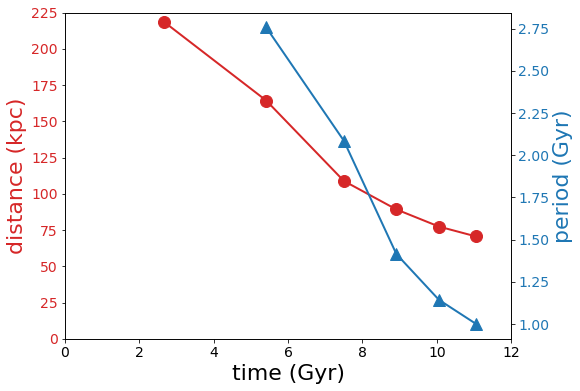
\includegraphics[scale=0.45]{decay1}\hspace{5mm} 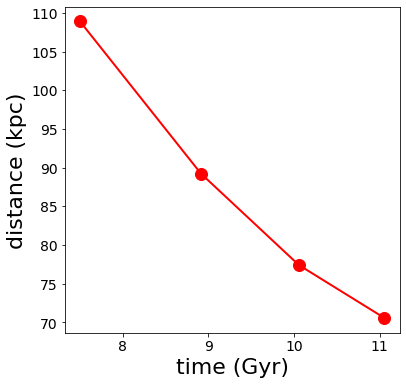
\includegraphics[scale=0.45]{decay2} \par}

The decay is non-linear, but by extrapolation from the last two points we can estimate 6.8 kpc/Gyr as an upper bound. From a 75 kpc separation, merger would take a further 11 Gyr (i.e. 22 Gyr from the start of the sim). A linear fit to all the apocenters beyond 6 Gyr gives a faster decay, with merger happening after about 6-7 Gyr.

\end{document}
